\setAuthor{Mihkel Heidelberg}
\setRound{piirkonnavoor}
\setYear{2008}
\setNumber{G 1}
\setDifficulty{1}
\setTopic{Staatika}

\prob{Pendel}
Otsast kinnitatud varras saab pöörelda ümber horisontaaltelje ühes tasandis. Varda otsa on kinnitatud koormis massiga $m$. Varda pikkus on $l$. Varda kinnitusele mõjub hõõrdest tingitud pidurdav jõumoment $M$. Millistes nurkade vahemikes võib olla varras paigal (vt joonist)? Arvestada, et $mgl > M$.
\begin{center}
	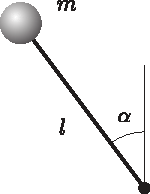
\includegraphics[width=0.3\linewidth]{2008-v2g-01-yl}
\end{center}

\hint
Kangi kriitilise nurga korral kehtib varda jaoks jõumomentide tasakaal.

\solu
Koormisele mõjub raskusjõu moment $mgl\sin \alpha$. Kang püsib paigal, kui see on väiksem hõõrdejõu momendist $M$, seega $mgl\sin \alpha < M$, millest $\sin \alpha < \frac{M}{mgl}$.
\probend